\section{Einleitung}

Der Versuch V14 umfasst die Anwendung des Verfahrens der Tomographie mittels
$\gamma -$Strahlung. Das Ziel des Versuches ist es die materielle Zusammensetzung
zwei bekannter, sowie einem unbekannten Objekt zu untersuchen.

\section{Theorie}

Die Tomgraphie ist ein bildgebendes Verfahren, welches auf dem Prinzip der Absorption
basiert. Dabei wird ein Objekt von $\gamma -$Strahlung, oder auch
Teilchen wie Elektronen oder Neutronen durchdrungen.
Die Anfangsintensität $I_0$ und Endintensität $I\ua{f}$ werden vermessen, sodass die Absorptionskonstante
$\mu$ des durchdrungenen Materials bestimmt werden kann.
Die Intensitäten hängen über einen exponentiellen Zusammenhang mit der
Absorptionskonstate und der Materialdicke $d$ zusammen.

\begin{equation}
  I\ua{f} = I_0 \exp{-\sum_i\mui\cdot d_i}
  \label{eqn:absorption}
\end{equation}

Die Absorptionskonstate ist materialspezifisch, weshalb aufgrund ihres Wertes
auf das Material zurückgeschlossen werden kann.
Das einmaligen Durchführen des Verfahren gibt lediglich einen Eindruck von einem
Querschnittes des Objektes. Deshalb ist eine mehrfach Ausführung
mit verschiedenen Durchdringungsrichtungen notwendig, um das Gesamtobjekt zu vermessen.

Die Gleichung \eqref{eqn:absorption} kann umgestellt werden, sodass ein
Gleichungssystem der Form:

\begin{equation}
  \underline{\underline{A}} \cdot \vec{\mu} = \vec{I}
  \label{eqn:LGS}
\end{equation}

In dem Versuch wird ein $3 \times 3 \times 3$ Würfel untersucht.
Deshalb ist die Dicke der einzelnen Würfel $d_i$ gleich $d = \SI{1}{\centi\meter}$
für alle Einheitswürfel.
Das bedeutet, dass es insgesamt neun verschiedene Absorptionskonstanten $\mu_1, \mu_2, ... , \mu_9$
in einer Ebene des Würfels vorliegen. Dementsprechend werden mindestend neun
verschiedene Projektionen benötigt, um das Gleichungssytem \eqref{eqn:LGS}
zu lösen. Das Messverfahren wird durch eine Überbestimmung des
Gleichungssytems erhöht, weshalb anstelle der nötigen neun Projektionen
zwölf Projektionen gewählt werden.
Eine Darstellung der gewählten Projektionen ist in Abb. \ref{fig:projektionen}
zu sehen.

\begin{figure}[h]
  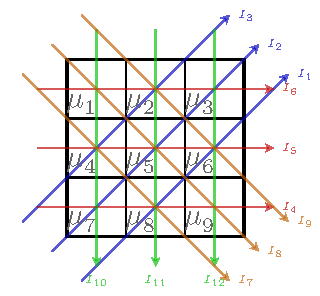
\includegraphics[width=\textwidth]{Pics/tikz-Projektionen.pdf}
  \caption{Schematische Darstellung der zwölf verwendeten Projektionen $I_1$ -- $I_{12}$.\cite[LuckyJosh]}
  \label{fig:projektionen}
\end{figure}

Die gewählten Projektionen erzeugen ein Gleichungssystem der Form:

\begin{align}

    d \cdot

    \begin{pmatrix}[r]
      0 & 0 & 0 & 0 & 0 & \sqrt{2} & 0 & \sqrt{2} & 0 \\
      0 & 0 & \sqrt{2} & 0 & \sqrt{2} & 0 & \sqrt{2} & 0 & 0 \\
      0 & \sqrt{2} & 0 & \sqrt{2} & 0 & 0 & 0 & 0 & 0 \\
      0 & 0 & 0 & 0 & 0 & 0 & 1 & 1 & 1 \\
      0 & 0 & 0 & 1 & 1 & 1 & 0 & 0 & 0 \\
      1 & 1 & 1 & 0 & 0 & 0 & 0 & 0 & 0 \\
      0 & 0 & 0 & \sqrt{2} & 0 & 0 & 0  & \sqrt{2} & 0 \\
      \sqrt{2} & 0 & 0 & 0 & \sqrt{2} & 0 & 0 & 0 & \sqrt{2} \\
      0 & \sqrt{2} & 0 & 0 & 0  & \sqrt{2} & 0 & 0 & 0\\
      1 & 0 & 0 & 1 & 0 & 0 & 1 & 0 & 0 \\
      0 & 1 & 0 & 0 & 1 & 0 & 0 & 1 & 0 \\
      0 & 0 & 1 & 0 & 0 & 1 & 0 & 0 & 1 \\
    \end{pmatrix}

    \cdot

    \begin{pmatrix}[r]

      \mu_1 \\
      \mu_2 \\
      \mu_3 \\
      \mu_4 \\
      \mu_5 \\
      \mu_6 \\
      \mu_7 \\
      \mu_8 \\
      \mu_9 \\
      \mu_10 \\
      \mu_11 \\
      \mu_12 \\

    \end{pmatrix}

    =

    \begin{pmatrix}[r]

      I_1 \\
      I_2 \\
      I_3 \\
      I_4 \\
      I_5 \\
      I_6 \\
      I_7 \\
      I_8 \\
      I_9 \\
      I_10 \\
      I_11 \\
      I_12 \\

    \end{pmatrix}.

    \label{eqn:LGS_ausgeschrieben}

\end{align}

Aufrund des Überbestimmtheit von \eqref{eqn:LGS_ausgeschrieben} wird die
"Methode der kleinsten Quadrate" verwendet, wodurch \eqref{eqn:LGS_ausgeschrieben}
in eine Normalengleichung der Form $\left(\underline{\underline{A}}^T\underline{\underline{A}}\right)
\cdot \vec{\mu} = \left(underline{\underline{A}}^T\cdot\vec{I}\right)$ überführt wird.
Umgestellt nach $\vec{\mu}$ ergibt:

\begin{equation}
  \vec{\mu} = \left(\underline{\underline{A}}^T\underline{\underline{A}}\right)^{-1}
  \underline{\underline{A}}^T\cdot \vec{I}.
  \label{eqn:mu_umgestellt}
\end{equation}

Die Varianz des Vektors $\vec{I}$ ist durch eine Diagonalmatrix gegeben (vgl. \eqref{kovarianz_I}).

\begin{equation}
  \symup{V}[\vec{I}] = \text{diag}\left(\sigma_{I_1}^2, \sigma_{I_2}^2, ... , \sigma_{I_12}^2\right)
  \label{eqn:kovarianz_I}
\end{equation}

Daraus ergibt sich die Kovarianzmatrix von $\vec{\mu}$ zu:

\begin{equation}
  \symup{V}[\vec{\mu}] = \left(\underline{\underline{A}}^T \symup{V}^{-1}[\vec{I}] \underline{\underline{A}}\right)^{-1}.
  \label{eqn:kovarianz_mu}
\end{equation}

Damit muss $\vec{\mu}$ umgeschrieben werden zu:

\begin{equation}
  \vec{\mu} = \symup{V}[\vec{\mu}] \underline{\underline{A}}^T \symup{V}^{-1}[\vec{I}] \cdot \vec{I}.
\end{equation}

\section{Durchführung}



\begin{figure}[h]
  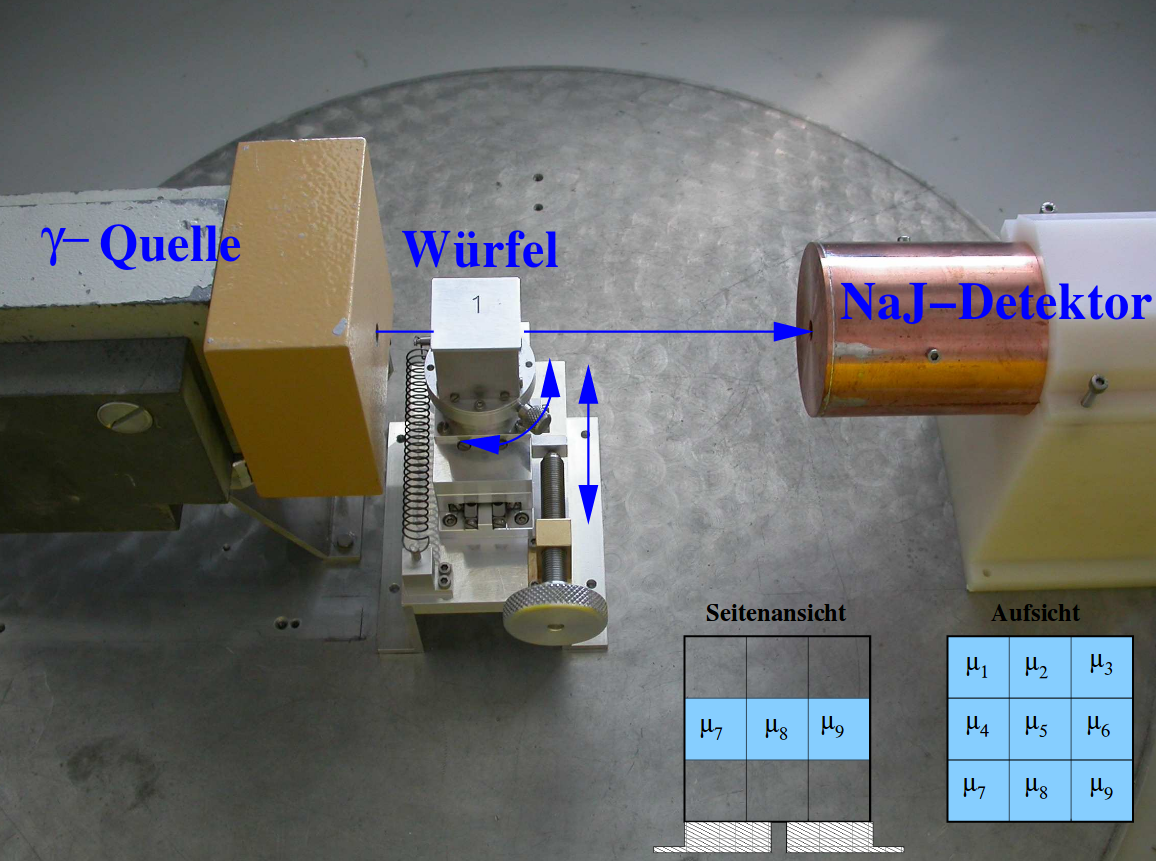
\includegraphics[width=\textwidth]{Pics/Aufbau.png}
  \caption{Verwendeter Veruschsaufbau. Nahaufnahme der Messaparatur.}
  \label{fig:aufbau}
\end{figure}
